\section{Introduction}
The \textrm{Dusk} network makes use of a decentralized and privacy-oriented digital currency that evolves the CryptoNote protocol\cite{CryptoNote} through the groundbreaking discoveries in the field of Byzantine consensus and pseudo-random functions of world renown cryptographers such as Silvio Micali, Michael Rabin, Alexander Yampolskiy and Evgeniy Dodis. \textrm{Dusk} radically departs from any other blockchain by employing an adaptive consensus mechanism, called Segregated Byzantine Agreement (or SBA{$\large\star$}), which does not require the computational intensity of proof-of-work and is a fairer alternative to proof-of-stake. Built on such consensus algorithm, \textrm{Dusk} is poised to be the first to simultaneously achieve previously conflicting goals of guaranteeing transaction untraceability and unlinkability, safeguarding user privacy, reaching transactional "finality" after a bound number of rounds within a single block election and achieving virtually unbounded user scalability without any significant performance degradation.

The \textrm{Dusk} network requires a heightened security setup designed specifically to:

\begin{enumerate}
\item Obfuscate IP addresses of the communicating peers
\item Prevent linkability and traceability of accounts
\item Guarantee network performance
\item Implement efficient payment mechanism for high QoS applications such as secure and anonymous voice calls
\end{enumerate}

An important difference with CryptoNote, is that \textrm{Dusk} does not make use of proof-of-work mining and therefore drops completely CryptoNight and deviates substantially from the hashing algorithms therein adopted. In particular, \textrm{Dusk} uses what we call \hyperref[sec:SBA]{Segregated Byzantine Agreement} (SBA$\large\star$) protocol which enhances classic BA$\large\star$ by implementing specific measures to protect peer privacy. SBA$\large\star$ has been developed specifically to power the \textrm{Dusk} Blockchain and help meeting the aforementioned requirements. These efforts do not solely relate to the application layer but extend to the networking layer as well. This is why the \textrm{Dusk} protocol makes use of:

\begin{itemize}
\item \textbf{Stealth addresses}: to protect transaction recipient anonymity
\item \textbf{RingCT signature}: to protect transaction sender's identity
\item \textbf{Anonymous Network Layer}: to protect the IP address of the network peers; to provide secure data transfer mechanism; to implement off-line data retrieval strategy; to power the anonymous gossip network for transaction propagation and verification
\item \textbf{Non-Interactive Verifiable Secret Sharing Scheme}: to conceal all but highest priority time-locked transactions from the participants to the Block Generation sortition
\item \textbf{Cryptographically Committed Provisioners}: to protect the information about stake; to implement a division of responsibilities between Block Generators and the electable Block Voters and Verifiers; to boost network efficiency by acting as state channel guarantors; to incentivise participation to the network; to protect the balance information of transacting nodes; to prepare SBA$\large\star$ for future expansion with non-balance and non-payment related weights such as storage contributed to the network (as in proof-of-storage), availability expressed in elapsed time since joining the network (as in proof-of-idle), etc.
\end{itemize}

\section {Preliminaries}

\subsection{Diffie-Hellman Hardness Assumption}

In any group, a discrete logarithm $log_b\space$ a is a number x $\in \mathbb{Z}$ such that $b^x = a$. 

Most of the cryptographic building blocks related to this work are linked to the Diffie-Hellman assumption which uses the hardness of discrete logarithms in cyclic groups \cite{CyclicGroup}. Considering a multiplicative cyclic group $\mathbb{G}$ of order $p$ and generator \cite{Generator} $g$, we can formulate the following assumption: given $g^a$ and $g^b$ for uniformly and independently chosen $a$ ,$b$ $\in \mathbb{Z}_p$ then $g^{ab}$ performs like a random element in $\mathbb{G}$ of order $p$.

As a consequence of such assumed randomness, the Decisional Diffie-Hellman (DDH) Problem relates to distinguishing the following two probability distributions:

\begin{itemize}
\item ($g^a, g^b, g^{ab}$) $\forall \space a,b \in \mathbb{Z}\\$ // $\small (g^a, g^b, g^{ab}) \textrm{ are defined as a Diffie-Hellman Tuple}$
\item ($g^a, g^b, g^{c}$) $\forall \space a,b,c \in \mathbb{Z}$
\end{itemize}

\subsection{Hiding Recipients: Stealth Addresses}
Inspired by the CryptoNote white-paper\cite{CryptoNote}, stealth address technology is at the basis of \textrm{Dusk} recipient hiding technique. Already widely tested in other privacy-oriented digital currencies, it is the proven choice for concealing the true recipient address of a transaction while keeping uniqueness within the context of the ledger (meaning no other address can be linked to a stealth address). Additionally, a derivation of an unbound number of receiving addresses is also possible without any of them allowing traceability back to the recipient's main address. As an anonymous key agreement protocol, \textrm{Dusk} uses the Elliptic Curve Diffie-Hellman (ECDH) due to the desired property of allowing two parties to generate a shared secret by solely knowing each other's public key, and the generator point of the Elliptic Curve used in the Twisted Edward equation. Following is a detailed explanation of how \textrm{Dusk} implements Stealth Address technology. 

\subsubsection{Elliptic-Curve Cryptography}

The system makes use of Elliptic-Curve Cryptography (ECC), hence approaching public-key cryptography through the algebraic structure of elliptic curves and thus allowing for the creation of smaller and more efficient cryptographic keys. ECC gives the same security levels of, for example, RSA, but using a much smaller security key.

The structure of an elliptic curve is a plane curve satisfying the equation $y^2=x^3+ax+b$, which returns us the graph in Figure \ref{fig:elliptic}.

\begin{figure}
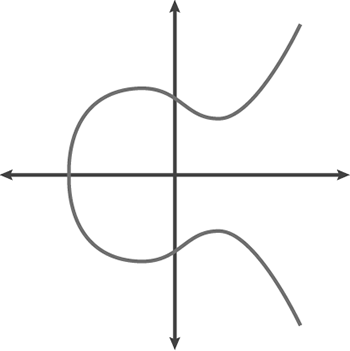
\includegraphics[height=1in, width=1in]{elliptic_bn}
\caption{A generic elliptic curve}
\label{fig:elliptic}
\end{figure}

In ECC, a Galois Field is created by taking the modulo of all points using a large prime number, creating a finite number of values for the used equation. The following axioms are furthermore taken into account:

\begin{enumerate}
\item A point can't be multiplied or divided by another point.
\item Any point on the curve can be added or subtracted to another point (or itself).
\item Adding a point to itself allows for scalar multiplication.
\end{enumerate}

\subsubsection{Private and Public Keys}

The \textrm{Dusk} Blockchain utilizes an \textit{Ed25519} curve, which is a Twisted Edwards curve with the following Elliptic Curve Parameters:

$q$ : a prime number; $q=2^{255}-19$ ; \textit{This is the number of points in the curve.}

$d$ : an element of $\mathbb{F}_q$; $d=-121665/121666$; \textit{Value used in the curve equation below}

$E$ : an elliptic curve equation; $-x^2+y^2=1+dx^2y^2$; \textit{The Twisted Edwards curve/equation we are using}

$G$ : a base point; $G=(x, -4/5)$; \textit{The}\textbf{**generator**} \textit{point. This is a base - starting point used for all Elliptic modulo operations.}

$l$ : a prime order of the base point; \\\space\space\space\space$l=2^{252}+27742317777372353535851937790883648493$ ;\\ \textit{The order of the base point} $G$\textit{. This defines the maximum size of scalars and the maximum number of points that can be used.}

$\mathcal{H}_s$: a cryptographic hash function $\{0,1\}^*\rightarrow\mathbb{F}_q$;

$\mathcal{H}_p$: a deterministic hash function $E(\mathbb{F}_q)\rightarrow E(\mathbb{F}_q)$;

All private and public keys in \textrm{Dusk} will be using 64 hex characters.

\subsubsection{Accounts and Addresses}

The following procedure will be used to create an address.

\begin{enumerate}
\item  We pick a random /textit{private spend key}, by generating 256 random bits, and reducing$\mod l$. We call this $b$.
\item  $b$ is hashed with hashing algorithm $H$(\textit{Keccak\_256}). We interpret the result of the hashing as an integer, reduce it $\mod l$ as before. We call this key $a$.  
\item  We generate our public spend and view keys $B=bG$ and $A=aG$
\item  We hash (network prefix (0xEF) + $B$ + $A$) with $H$.
\item  Append the first 4 bytes of this operation to (prefix + $B$ + $A$), obtaining a 69 bytes value (1 + 32 + 32 + 4)
\item  Convert this to \textit{cnBase58}.
\end{enumerate}

We will explain how stealth addresses work by first going trough a brief explanation about key exchanges on an ECC scenario, in the next section.

\subsubsection{The Elliptic Curve Diffie-Hellman}

The Elliptic Curve Diffie-Hellman (ECDH) is an anonymous key agreement protocol, a variant of the Diffie-Hellman protocol adapted to work with Elliptic-Curve Cryptography.

Thanks to ECDH, two parties can generate a shared secret over an unsecured connection only by knowing each other's public keys, and the generator point of the Elliptic Curve used in the ECC equation.

To demonstrate this, we will use Alice (with private key a and public key A=aG) and Bob (with private key b and public key B=bG). (Where G is the generator point)

As previously stated, points on a curve can be added together, and Alice could calculate a point C = A + B, but this could also be potentially done by anyone eavesdropping the conversation, since A and B are publicly available.

Now, let's remember that A and B are points on the elliptical curve, and that we can add a point to itself.

Alice can now calculate a new point D=aB,  and Bob can get D'=bA.

We can now prove that D=D', and thus Alice and Bob share a secret by operating on ECC and knowing each other's public keys and the generator point G:

\begin{enumerate}
\item Given a common generator point G;
\item Alice has a=5, A=5G (private and public keys)
\item Bob has b=7, B =7G
\item a · b = 35
\item Alice computes D=aB=5B=5·7G=35G
\item Bob computes D'=bA=7A=7·5G=35G
\item D=D'
\end{enumerate}

Point D has a corresponding scalar d, in the example above equal to 35, which is a shared secret between Alice and Bob

\subsubsection{Stealth Addresses}

Let's consider the diagram in Figure \ref{fig:cryptodg} from the CryptoNote whitepaper.

\begin{figure}
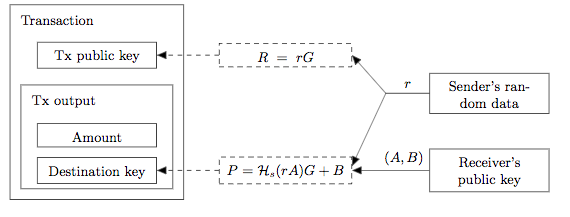
\includegraphics[height=1in]{M42G4Fy}
\caption{A \textit{stealth transaction}}
\label{fig:cryptodg}
\end{figure}

The \textit{Dual-key Stealth Address} $P$ is defined as $P=\mathcal{H}_s(rA) \cdot G+B$. The link-ability of the Stealth Address is achieved by using a combination of spend/view-keys, without actually allowing a spending transaction to take place. Let's now assume that Alice has a private \textit{spend-key} $z$ and a private \textit{view-key} $y$. We call her public \textit{spend/view-keys} $Z,Y$. On the other side, Bob's public keys are $A$ and $B$, with Bob's private keys $a$ and $b$ unknown to Alice. In order to build a stealth address, Bob needs to compute $r$ (an arbitrary random scalar chosen by Alice) and $R$ as the corresponding ECC point such as $R=rG$. $r$ is not being shared with anyone and can be discarded after its use - unless Alice wants to prove that she sent a transaction to Bob to an external party. $R$ is added to the transaction so that it can be seen by everyone. A new $r$ is calculated for each transaction, since reusing it in the computation of the Stealth Address, would result in a collision. Therefore, given the equation above: $P=\mathcal{H}_s(rA)G+B$, a Stealth Address can be constructed as follows.

\begin{enumerate}
\item P : the Stealth Address where the funds will be sent
\item $\mathcal{H}_s$ : a Hashing Algorithm returning a scalar value
\item r : the random scalar chosen by Alice
\item A : Bob's public view-key
\item G : The standard Ed25519 base point
\item B : Bob's public spend-key
\end{enumerate}

Alice calculates point D from ECDH using a randomly chosen r and Bob's public key A.

Bob computes D independently from Alice, due to the properties of ECDH.

Alice computes the scalar $f=\mathcal{H}_s(D)$ - (this hashing step creates unlinkability between Bob's address and the new stealth one) and calculates F=fG, and P = F + B (Bob's public spend-key).

Now, in order to check if he is the transaction's recipient, Bob:

\begin{enumerate}
\item Calculates D' using R as propagated with the transaction (The equality D = D'=aR is still unproven).
\item Calculates f'=$\mathcal{H}_s(D')$
\item Calculates F'=f'G
\item Calculates P'=F'+B
\end{enumerate}

If P'=P, then Bob knows the transaction was intended for him, and can retrieve it like this:

(Bob has to compute the secret key associated with the transaction)

\begin{enumerate}
\item Bob knows f' (computed above), and derives xf'+b  (Bob's private spend key)
\item Knowing that P=xG, we got P=xG=(f'+b)G
\item Bob then has to check if the transaction on P is spent, Bob computes a key-image and checks on the blockchain if the image linked to that transaction has been spent. Image I=x$\mathcal{H}_p(P)$
\item Bob can then sign a new transaction using x
\end{enumerate}

\subsection{Obfuscating Sender}

Ring Signatures are an efficient, established way to obfuscate the input of a transaction by making use of a sender's account keys and a number of decoy keys (called \textit{outputs}) taken directly from the blockchain, using a triangular distribution method. The technology finds its roots in the early days of blockchain research, as Satoshi Nakamoto himself was hypothesizing back in 2010:


\blockquote{Crypto may offer "key blinding". I did some research and it was obscure, but there may be something there. "Group signatures" may be related.} \footnote{https://bitcointalk.org/index.php?topic=770.msg9074\#msg9074}

The procedure allows one of the members of the \textit{ring} to sign messages on behalf of the whole group, and by doing so it renders it infeasible to know exactly which member signed. (Figure \ref{fig:ringsig})

\begin{figure}
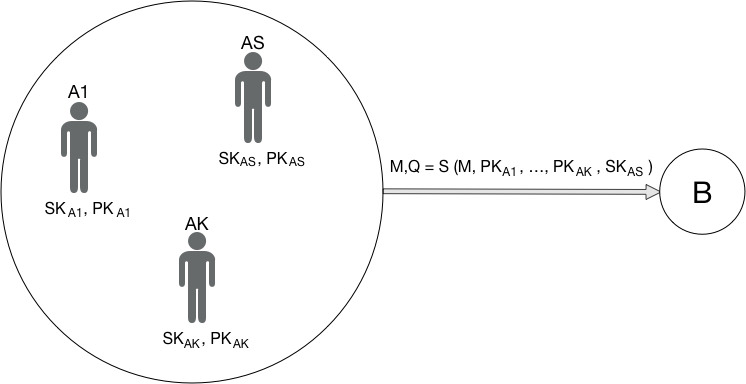
\includegraphics[scale=0.35]{ringsig}
\caption{A \textit{ring signature transaction}}
\label{fig:ringsig}
\end{figure}

In a group signature procedure, there is no central management or setup - all the signer needs is the public keys of the members she chooses to be part of the ring.

Each signer is associated with a public key $PK_x$ and a corresponding private key $SK_x$. A ring signature scheme is defined by two procedures:

\begin{itemize}
\item $\textrm{ringSign}(M, PK_1, PK_2, ..., PK_r, s, SK_s)$: which is a method for computing the ring signature Q, which gets the message M, the public keys of the ring members, and the private key of the message signer.
\item $\textrm{ringVerify}(M,Q)$: which is a procedure to verify the signature Q, which gets message M and signature Q as arguments, and returns a boolean (correct / not correct) as output.
\end{itemize}

\subsubsection{Signature Generation}

Having a message $m$ and its own private key $SK_s$, together with a sequence of ring member's public keys, signer $A_s$ can create a signature as follows:

\begin{enumerate}
\item Computes a key $k=h(m)$, where $h$ is a collision-resistant hash function.
\item Chooses a random $v$
\item Chooses a random $x_i$ and computes $y_i=g_i(x_i)$
\item Solves for $y_s$ the equation containing the \textit{Combining function} $C_{k,v}(y_1,y_2,...,y_r) = v$
\item Finds $x_s$ knowing its own $SK_s$: $x_s=g_s^{-1}$
\item Creates a ring signature: $v; x_1, x_2, ..., x_r$
\end{enumerate}

\subsubsection{Signature Verification}

A verifier can confirm a ring signature as follows, having the collection of the member's *public keys:*

\begin{enumerate}
\item Compute, for each $x_1$, $y_1=g_i(x_1)$
\item Computes $k=h(m)$
\item Confirms the equation $C_{k,v}(y_1,y_2, ..., y_r)=v$ for values of $y_i$
\item If the equation is correct then the signature is valid, otherwise it's not.
\end{enumerate}

\subsubsection{Ring Confidential Transactions}

Blockchains such as Monero use a particular breed of ring signatures called Ring Signature Confidential Transactions (\textit{RingCT}), where the privacy is taken one step further by not only giving full anonymity at the sender level (as explained above), but also on the amount spent and destination.

The RingCT technology makes the payment virtually unlinkable to the original spender, it is fast, and it also  conceals the amount being transferred. Confidential Transactions include cryptographic proof that, given a set of input amounts, proves that their sum equates the output amounts, without revealing them. In practice, if \textit{Alice} has an output of 15 \textrm{Dusk} and wants to send \textit{Bob} 7 \textrm{Dusk}, she will have to spend the output in its entirety on transaction $T$, and then send the change (8 \textrm{Dusk}) back to herself. (Figure \ref{fig:ringtx})

\begin{figure}
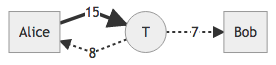
\includegraphics[scale=0.7]{ringtx}
\caption{A \textit{ring stealth transaction}}
\label{fig:ringtx}
\end{figure}

This commitment is represented by the formula: 

$R_{ct}=xG + aH(G)$

In the formula, $a$ is the amount sent out in the transaction, $x$ is a computed random value. By publishing the value of $R_{ct}$ to the network as an output, the network will be able to verify the legitimacy of the submitted transaction. This technology goes on top of the already untraceable (Stealth) addresses used by the \textrm{Dusk} blockchain, and anonymous networking used to give full anonymity to the nodes involved.

In the \textrm{Dusk} Network, RingCT is used by default for all transactions except those used to participate to the sortition for Block Generator (which are normally \textit{ring signed}). This is merely a detail, though, considering that an external observer would not be able to tell these two kind of transactions apart from each other.

\subsubsection{Future Development: Bulletproof Transactions}

Initially, non-interactive proof of knowledge based on [Fiat-Shamir heuristic \cite{Shamir} have been taken into consideration in order to conceal transaction information such as sender and amount. However, it quickly appeared that technologies developed on top of its concept such as zk-SNARKs \cite{zcash} require prohibitive computational power and time of processing for transaction generation. Even the more recent zk-STARKS \cite{starks}) proved impractical to integrate in \textrm{Dusk} because of the problematic hurdle of needing extremely bulky verification proof (as big as several hundreds of kilobytes), although solving the problematic reliance on a trusted third-party for system setup and being substantially simpler than zk-SNARKS in terms of cryptographic primitives (they do not make use of Elliptic Curves, nor Public Key cryptography). 

The most promising advancement in the field of transaction confidentiality is probably given by the so-called Bulletproof Transactions \cite{bulletproofs}, which would appear to provide a substantial improvement over RingCT in terms of cryptographic proof size. At the time of this writing, first tests show a tenfold reduction in size and verification times (although still not reaching the same level of efficiency if compared to a zk-SNARK proof). Given the "pluggable" nature of \textrm{Dusk} core, the underlying software for transaction generation will be kept flexible through a plugin architecture in order to facilitate the adoption of a future implementation of Bulletproof Transactions as soon as an emerging library proves stable enough for integration.

\subsection{Cryptographic Accumulator}
\label{sec:Cryptographic-Accumulator}
The set of algorithms known as cryptographic accumulators have been developed to allow hashing of a finite and potentially large set of values into a single succinct value, called the Accumulator. The algorithm enables efficient computation of a witness for every accumulated input that proves its membership in the Accumulator. A dynamic Accumulator is a special kind of Accumulator which permits efficient input addition and deletion where the computation costs of these operation is independent on the number of values added or deleted. As such, it is a space and computational time efficient data structure initially developed for testing membership. 

Formally, a dynamic Accumulator is a tuple of algorithms defined as follows:

\begin{itemize}
\item  $\textrm{Generate}(1^k)\rightarrow (sk_{acc}, pk_{acc})$: Given a security parameter $k$ return a (private, public) key pair. Notice that the parameter $k$ is sensitive information (trapdoor) which could deterministically recreate the private key  
\item  $\textrm{Eval}((sk_{acc}, pk_{acc}), \chi) \rightarrow (acc_\chi, aux)$: Probabilistic algorithm that gets the key pair and a set $\chi$ to be accumulated and returns the Accumulator and some auxiliary data
\item  $\textrm{WitnessCreate}((sk_{acc}, pk_{acc}), acc_\chi, aux, x_i)\rightarrow wit_x \lor \bot$: Creates a witness $wit_x$ if $x_i \in \chi$, $\bot$ otherwise
\item  $\textrm{Verify}(pk_{acc}, acc_\chi, wit_x, x_i)\rightarrow wit_x\space \textrm{is a witness for }x_i$: This is the actual membership verification
\item  $\textrm{Add}(sk_{acc}, pk_{acc}, acc_\chi, aux, y_i)\rightarrow acc_{\chi'} \lor \bot$ : If the element $y_i$ is not already in the set $\chi$, returns the updated Accumulator $acc_{\chi'}$ with $\chi' \leftarrow \chi \space \bigcup \space \{y_i\}$ 
\item  $\textrm{Delete}(sk_{acc}, pk_{acc}, acc_\chi, aux, y_i)\rightarrow acc_{\chi'} \lor \bot$ : If the element $y_i$ is in the set $\chi$, returns the updated Accumulator $acc_{\chi'}$ with $\chi' \leftarrow \chi \space \backslash \space \{y_i\}$
\item  $\textrm{WitnessUpdate}((sk_{acc}, pk_{acc}), wit_x, aux, x_i)\rightarrow wit'_x \lor \bot$: Updates the witness for $x_i$ in case it has been added or deleted ($aux$ describes which of the two)
\end{itemize}

Different technologies exist that implement Accumulators with different level of computational efficiency and security requirements. Currently, \textrm{Dusk} is experimenting to achieve the best trade-off between a decentralized choice and efficiency of Accumulator technology. Following are the technologies under evaluation.

\subsubsection{RSA Accumulators}

Abundant literature has been developed regarding many different Accumulators, particularly the so-called RSA Accumulators. Considering \textit{strong RSA setting}, RSA Accumulators (e.g. Carmenish's and Lysyanskaya's Dynamic RSA Accumulator \cite{accumulators}) are based on one-way RSA function for a suitably calculated $N =pq$ where $p$ and $q$ are sample primes with polynomial dependence on the security parameter $k$ and therefore are effectively the Accumulator's \textit{trapdoors} which need to be \textbf{destroyed} immediately after parameters are generated. As an alternative, the employment of RSA-2048 could be used to circumvent the need for developers to know the security parameters and act as trusted party, considering that the related security parameter $k$ is claimed to be destroyed and no factoring solution to the RSA-2048 number has been found for the past 25 years \footnote{https://en.wikipedia.org/wiki/RSA\_Factoring\_Challenge}, despite a \$200,000 incentive offered.

$acc_\chi \leftarrow g^{a} mod\space N$ // The set of members $a =\{a_1, .., a_n\}$ is compactly represented by the Accumulator
$acc_\chi = g^{\prod{a \in \chi}}\\wit_i \leftarrow g^{(a_1, .., a_{i-1}, a_{i+1}, .., a_n)} mod\space N$

\subsubsection{Expressive Bilinear Accumulator}

Under such security assumption, dynamic Accumulator schemes from \textit{bilinear pairings} have been developed in the literature. Among those, an expressive \textit{zero-knowledge} set Accumulator has been formalized by Zhang, Katz and Papamanthou \cite{zeroaccum} capable of providing succinct proofs for a large collection of operations over accumulated sets, among which it is of particular interest the $\textrm{SUM}$ operation, which could find application for rapid and zero-knowledge calculation of accumulated \hyperref[sec:Cryptographically-Committed-Provisioners]{Provisioners stakes}.

However, similarly to RSA, bilinear pairing Accumulators present also the drawback of relying on the security parameter $k$.

\subsubsection{Elliptic Curve Multiset Hash}

Shepard, Tibouchi and Aranha \cite{ecmh} teach of a new and efficient method to "\textit{associate a hash value to arbitrary collections of objects (with possible repetitions) in such a way that the hash of the union of two collections is easy to compute from the hashes of the two collections themselves:  it is simply their sum under a suitable group operation}". This association is the basis for an Elliptic Curve Multiset Hash which constructs a homomorphic multiset hashing on top of efficient \textit{BLAKE2} hash function and binary elliptic curve encoding. This allows for incremental/parallel computation of a hashing function for various applications including efficiently testing for subgroup membership. This makes ECMH an appealing alternative to the other known algorithms to construct Accumulators, especially since the method is unencumbered with the necessity of a trusted setup.

